\documentclass{article}
\usepackage[utf8]{inputenc}
\usepackage{fancyhdr}
\usepackage[margin=1.0in]{geometry}
\usepackage{amsmath,comment}
\usepackage{changepage}
\usepackage{graphicx}
\usepackage[inline]{enumitem}
\usepackage{enumitem}
\pagestyle{fancy}
\chead{Math 121 - Equations of tangent lines}
\renewcommand{\baselinestretch}{1.5}
\makeatletter
\newcommand{\inlineitem}[1][]{%
\ifnum\enit@type=\tw@
    {\descriptionlabel{#1}}
  \hspace{\labelsep}%
\else
  \ifnum\enit@type=\z@
       \refstepcounter{\@listctr}\fi
    \quad\@itemlabel\hspace{\labelsep}%
\fi}
\makeatother
\begin{document}
\begin{enumerate}
\item If you have a line with slope $m$, through the point $(x_1,y_1)$, what is the equation of the line?
\item Find the equation of the tangent line to the curve $y = 2x^3 - x + 4$ when $x = 1$.
\begin{figure}[h]
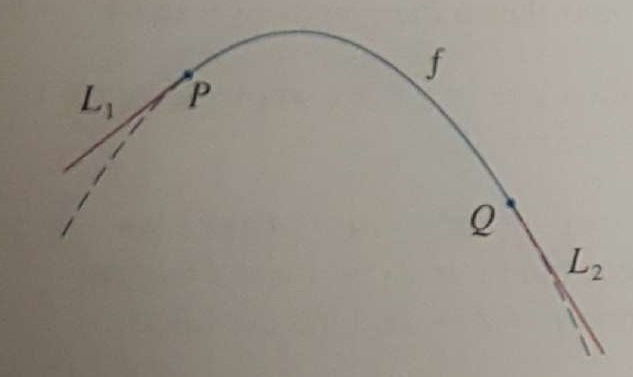
\includegraphics[scale=.8]{roll.jpg}
\centering
\end{figure}
\item You are building a roller coaster. You decide to make the slope of the ascent 0.8 and the slope of the drop -1.6. You decide to connect these two straight stretches $ y = L_1(x) $ and $ y = L_2(x) $ with part of a parabola $f(x) = ax^2 + bx + c $, where $ x $ and $ f(x) $ are measured in feet. For the track to be smooth there can't be abrupt changes in direction, so you want the linear segments $ L_1 $ and $ L_2 $ to be tangent to the parabola at the transition points $ P $ and $ Q $. (See the figure.) To simplify the equations, you decide to place the origin at $ P $.

\begin{enumerate}[label=(\alph*)]
\itemsep0em
\item Sketch some axes on the picture above. The point (0,0) should be at $P$, and the $x$-coordinate of $Q$ should be 100.

\item Based on the axes we drew, the horizontal distance between $ P $ and $ Q $ is 100 ft. We're trying to find our function $f(x)$. We know that $f'(x) =0.8$ at $P$, but we chose $P$ to have an $x$ value of 0. Therefore, $f'(0) = 0.8.$ Similarly, $f'(100) = -1.6$, to make the connection work at $Q$.

Write equations in $ a $, $ b $ and $ c $ that will make these derivatives agree. This will ensure that the track is smooth at the transition points.

\item Solve the equations in part (b) for $ a $, $ b $, and $ c $ to find a formula for $ f(x) $.
\item We can find the equation for $L_1(x)$ and $L_2(x)$. The slopes are given above, and our choice of coordinates gives $x$ values for $P$ and $Q$. Use what you found in part (c) to find the $y$ values for points $P$ and $Q$, and use that information to get the equations for $L_1(x)$ and $L_2(x)$.

\item Use technology to plot $ L_1 $, $ f $, and $ L_2 $ to verify graphically that the transitions are smooth.

\end{enumerate}
\end{enumerate}
\end{document}